%\documentclass[a4paper,11pt]{article}
\documentclass[a4paper,11pt]{report}
\usepackage{import}
%\usepackage{projectstyle}

%de naam hier is de naam van de file in de sty folder niet de naam van providespackage
\usepackage{sty/1loadrequiredpackagesatveryfirst}
\usepackage{sty/2metadata}
\usepackage{sty/3tocstyle}
%\usepackage{sty/4appendixstyle}
%\usepackage{sty/5colorstyles}
\usepackage{sty/6sectionsstyle}
\usepackage{sty/7newcommandsfilip}
\usepackage{sty/8glossariesstyle}
\usepackage{sty/9imagesstyle}
\usepackage{sty/10liststyles}
\usepackage{sty/11headerfooterstyle}
%\newcommand\TestAppExists[3]{#2}
\usepackage{sty/12mathstyles}
\usepackage{sty/13customstylesfromothersites}
\usepackage{sty/14stylesforalgoritmsandsourcecode}
\usepackage{lipsum}
%\usepackage{sty/15stylefortodonotes}
%\usepackage{sty/}
%\usepackage{sty/}
%\usepackage{sty/}
\usepackage{mdframed}
\usepackage{titletoc} % Required for manipulating the table of contents
\usepackage[hidelinks,
            colorlinks=false, %links krijgen kleuren of niet
            % breaklinks=true,
            % bookmarks=true,
            % bookmarksnumbered,
            % bookmarksopen=false,
            % urlcolor=webbrown,
            % linkcolor=red, %bepaalt de kleur van de links
            % citecolor=webgreen, % Link colors
            pdftex,
            pdfauthor={\theauthor}, % PDF Author
            pdftitle={\thetitle},% PDF title
            pdfsubject={\thesubject}, % PDF Subject
            pdfkeywords={\thekeywords}, % PDF Keywords
            pdfproducer={\thepdfproducer}, % PDF producer
            pdfcreator={\thepdfcreator} % PDF Creator
            ]{hyperref} %It gives LaTeX the possibility to manage links within the document or to any URL when you compile in PDF

\newcommand{\bfsp}{\renewcommand\labelitemi{$\bullet$}}


%\usepackage{minitoc} %Produce a table of contents for each chapter, part or section
%http://tex.stackexchange.com/questions/3001/list-sections-of-chapter-at-beginning-of-that-chapter
%http://www.ctan.org/pkg/minitoc
%
%
%\renewcommand{\mtctitle}{Inhoudsopgave}
%dit zet de "contents" string om in de string
%"inhoudsopgave" van het pakket minitoc
%\nomtcrule         % removes rules = horizontal lines


%\usepackage{makeidx}

%\usepackage{pdfpages}

%It prints out all index entries in the left margin of the text. This is quite useful for proofreading a document and verifying the index. For more information, see the Indexing section.

%https://en.wikibooks.org/wiki/LaTeX/Indexing

%\usepackage{showidx} %It prints out all index entries in the left margin of the text.

%\makeindex

%we have to define a bibliography style in the preamble
%\bibliographystyle{plain}

%\usepackage{booktabs}

%\usepackage{exsheets}

%\DeclareTranslation{Dutch}{exsheets-exercise-name}{Vraag}
%\DeclareTranslation{Dutch}{exsheets-question-name}{opgave}
%\DeclareTranslation{Dutch}{exsheets-solution-name}{Oplossing}

%\usepackage{caption}
%\usepackage{wrapfig}
%\titlespacing{\chapter}{0pt}{2ex}{1ex}
\titlespacing{\section}{0pt}{2ex}{1ex}
\titlespacing{\subsection}{0pt}{1ex}{0ex}
\titlespacing{\subsubsection}{0pt}{0.5ex}{0ex}
%\usepackage{subcaption}

\definecolor{gray75}{gray}{0.75}
\newcommand{\hsp}{\hspace{20pt}}

\titleformat{\chapter}[hang]
{\filright\normalfont\Huge\bfseries}
%{\chaptertitlename~\thechapter} {0.5em} {}
%{\chaptertitlename~\thechapter\hsp\textcolor{gray75}{|}\hsp} {0pt} {}
{\chaptertitlename~\thechapter\hsp\textcolor{gray75}{|}\hsp} {0pt} {#1}

%http://tex.stackexchange.com/questions/32317/adding-section-number-after-section-title-with-titlesec-package


%http://tex.stackexchange.com/questions/101502/chapter-number-and-title-in-one-row
%http://texblog.org/2012/07/03/fancy-latex-chapter-styles/
%http://ftp.isu.edu.tw/pub/Unix/CTAN/macros/latex/contrib/minitoc/minitoc.pdf
%

%\titleformat{\part}[display]
%{\vspace*{\fill}
%{\normalfont\huge\filcenter\bfseries}
%{\partname\ \thepart}
%{\partname} ==> print op pdf: "Deel"
%{\thepart} ==> print op pdf: " I en nieuwe line: Theorie
%{20pt}
%{\Huge}
%\titlespacing*{\part}{0pt}{0pt}{40pt}

%dit is voor de chapters
\newcommand\PartialTocChapter{%\vspace*{2pc}\hrule\vspace*{1pc}%
%\startcontents[chapters]\vbox{\bf\Large Inhoudsopgave }
\startcontents[chapters] % als je de lijn hierboven activeert, wordt onder threads en boven de lijn 
% inhoudsopgave geschreven
\printcontents[chapters]{}{1}{\setcounter{tocdepth}{1}}
\newpage
}%\vspace*{1pc}\hrule}

%dit is voor de parts
\newcommand\PartialTocPart{%\vspace*{2pc}\hrule\vspace*{1pc}%
\thispagestyle{fancy}

%The command \fancyhf{} clears the header and footer, otherwise the elements of the default "plain" page style will appear.
\fancyhf{}

%Prints the text included inside the braces on the right side of the header.
%\fancyhead[RE]{\textbf{\textit{\nouppercase{\leftmark}}}}

\fancyfoot[LF]{Filip Vanden Eynde~\copyright~2016}
\fancyfoot[RF]{Pagina \thepage \hspace{1pt} van \pageref{LastPage}} %plaats rechtsonder in de footer
\renewcommand{\footrulewidth}{1pt}
\renewcommand{\headrulewidth}{0pt}
\startcontents[parts]\vbox{\bf\Large Deel \thepart ~ inhoudsopgave}
\printcontents[parts]{}{0}{\setcounter{tocdepth}{1}}
%\setlength{\headheight}{15pt}
%\pagestyle{fancy}
%\renewcommand{\sectionmark}[1]{\markright{#1}{}}
%%The command \fancyhf{} clears the header and footer, otherwise the elements of the default "plain" page style will appear.
%\fancyhf{}
%\fancyhead[RH]{\textbf{\textit{\nouppercase{\leftmark}}}}
%\fancyhead[LH]{\textbf{\textit{\nouppercase{\rightmark}}}}
%
%%\fancyfoot[LF]{Copyright Filip Vanden Eynde}
%\fancyfoot[LF]{Filip Vanden Eynde~\copyright~2016}
%%http://sites.ieee.org/cec2015/for-latex-users/
%\fancyfoot[RF]{Pagina \thepage \hspace{1pt} van \pageref{LastPage}} %plaats rechtsonder in de footer
%
%%teken lijn boven footer
%\renewcommand{\footrulewidth}{1pt}


}%\vspace*{1pc}\hrule}

\definecolor{mybluei}{RGB}{0,173,239}
\definecolor{myblueii}{RGB}{63,200,244}
\definecolor{myblueiii}{RGB}{199,234,253}
\definecolor{myblue}{RGB}{0,0,122}

%\renewcommand\thepart{\arabic{part}}

\newcommand\partnumfont{% font specification for the number
  \fontsize{380}{130}\color{myblueii}\selectfont%
}
%http://tex.stackexchange.com/questions/159551/customizing-part-style-with-tikz/
\newcommand\partnamefont{% font specification for the name "PART"
 \normalfont\color{white}\scshape\small\bfseries


}

%The commands \partnumfont and \partnamefont are used to control the font attributes for the number and the label "Part". Feel free to make adjustments (fonts, sizes) according to your needs.
%

%http://tex.stackexchange.com/questions/266776/header-and-section-fancy-styles
%


%\titleformat{\part}
%  {\normalfont\huge\filleft}
%  {}
%  {20pt}
%  {\begin{tikzpicture}[remember picture,overlay]
%  \fill[myblueiii] %onderste gedeelte waarin de titel van de part instaat
%    (current page.north west) rectangle ([yshift=-13cm]current page.north east);
%  \node[
%  %bovenste gedeelte van part page style waar de I instaat.
%      fill=mybluei,
%      text width=2\paperwidth,
%      rounded corners=6cm,
%      text depth=18cm,
%      anchor=center,
%      inner sep=0pt] at (current page.north east) (parttop)
%    {\thepart};%
%  \node[
%      anchor=south east,
%      inner sep=0pt,
%      outer sep=0pt] (partnum) at ([xshift=-20pt]parttop.south)
%    {\partnumfont\thepart};
%  \node[
%      anchor=south,
%      inner sep=0pt] (partname) at ([yshift=2pt]partnum.south)
%  {\partnamefont DEEL};
%  \node[
%      anchor=north east,
%      align=right,
%      inner xsep=0pt] at ([yshift=-0.5cm]partname.east|-partnum.south)
%  {\parbox{.7\textwidth}{\raggedleft#1}};
%  \end{tikzpicture}%
%  }

\titleformat{\section}
  {\addtolength{\titlewidth}{2pc}\normalfont\Large\sffamily\bfseries}
  {\colorbox{myblueii}{\parbox{2cm}{\strut\color{white}\hfill\thesection}}}
  {1em}{#1}
  [{\titleline*[l]{\color{myblueii}\titlerule[2pt]}}]
  
\titleformat{\subsection}
  {\addtolength{\titlewidth}{2pc}\normalfont\large\sffamily}
    {\colorbox{myblueii}
        {\parbox{2cm}
            {\strut\color{white}\hfill\thesubsection}
        }
    }
  {1em}{#1}
  [
    {\titleline*[l]
        {\color{myblueii}\titlerule[2pt]}
    }
  ]

\usepackage{epigraph}
\usepackage{xpatch}
\usepackage{lmodern}

\newlength\ChapWd
\settowidth\ChapWd{\Huge\chaptertitlename} % Dees past het vak hoofdstuk 1 aan qua grootte


%
% Dit maakt de aanpassing aan de chapter pages
%http://tex.stackexchange.com/questions/122759/how-to-obtain-this-fancy-chapter-page-with-the-book-class
%
\titleformat{\chapter}[display]
  {\normalfont\filcenter\sffamily}
  {\tikz[remember picture,overlay]
    {
    \node[fill=mybluei,font=\fontsize{60}{72}\selectfont\color{white},anchor=north east,minimum size=\ChapWd]
      at ([xshift=-15pt,yshift=-15pt]current page.north east)
      (numb) {\thechapter};
    \node[rotate=90,anchor=south,inner sep=10pt,font=\huge] at (numb.west) {\color{mybluei}\chaptertitlename};
    }
  }{0pt}{\fontsize{33}{40}\selectfont\color{mybluei}#1}[\vskip10pt\Large***\vspace{50pt}]
\titlespacing*{\chapter}
  {0pt}{50pt}{10pt}


\makeatletter
\xpatchcmd{\ttl@printlist}{\endgroup}{{
\noindent\color{mybluei}\rule{\textwidth}{1.5pt}}\vskip30pt\endgroup}{}{}
\makeatother

\makeatletter
\xpatchcmd{\ttl@printlist}{\begingroup}{{
\noindent\color{mybluei}\rule{\textwidth}{1.5pt}}\vskip10pt\begingroup}{}{}
\makeatother


\begin{document}

%\glsaddall
%\import{./}{title.tex}

%\clearpage

%dit is voor de titelpagina
\import{./}{title2.tex}
%\clearpage


\newpage

%\thispagestyle{empty}
\pagestyle{empty}
%\dominitoc %initialization
%\dominitoc[n]% zorgt ervoor dat de titel "inhoudsopgave" verborgen wordt"
\tableofcontents

% Add “Page” above page numbers
%\addtocontents{toc}{~\hfill\textbf{Page}\par}

%\clearpage
\newpage

\part{Theorie}

%dees werkt zeker wel
%\startcontents[level-0]
%\printcontents[level-0]{}{0}{\setcounter{tocdepth}{2}}
%
%
\PartialTocPart
%\import{sections/lessen/hoofdstuk3/}{deel1.tex}

%\setcounter{chapter}{3}
\chapter{Threads}



\PartialTocChapter

%\startcontents[level-1]
%\printcontents[level-1]{}{1}{\setcounter{tocdepth}{1}}

%\startcontents[chapters]
\setlength{\headheight}{15pt}
\pagestyle{fancy}
\renewcommand{\sectionmark}[1]{\markright{#1}{}}

%The command \fancyhf{} clears the header and footer, otherwise the elements of the default "plain" page style will appear.
\fancyhf{}
\fancyhead[RH]{\textbf{\textit{\nouppercase{\leftmark}}}}
\fancyhead[LH]{\textbf{\textit{\nouppercase{\rightmark}}}}
\fancyfoot[LF]{Filip Vanden Eynde~\copyright~2016}
\fancyfoot[RF]{Pagina \thepage \hspace{1pt} van \pageref{LastPage}} %plaats rechtsonder in de footer
\renewcommand{\footrulewidth}{1pt}
\renewcommand{\headrulewidth}{1pt}

\section{Overview}
\lipsum
%\import{sections/lessen/hoofdstuk4/}{deel1.tex}
\section{Multicore Programming}
\lipsum
%\import{sections/lessen/hoofdstuk4/}{deel2.tex}
\section{Multithreading Models}
\lipsum
%\import{sections/lessen/hoofdstuk4/}{deel3.tex}
\section{Thread Libraries}
\lipsum
%\import{sections/lessen/hoofdstuk4/}{deel4.tex}
\section{Implicit Threading}
\lipsum
%\import{sections/lessen/hoofdstuk4/}{deel5.tex}
\section{Threading Issues}
\lipsum
%\import{sections/lessen/hoofdstuk4/}{deel6.tex}
\section{Operating System Examples}
\lipsum
%\import{sections/lessen/hoofdstuk4/}{deel7.tex}


%%%%%%%%%%%%%%%%%%%%%%%%%%%%%%%%%%%%%%%%%%%%
%\stopcontents[level-1]

\chapter{Process Synchronization}

%\minitoc% Creating an actual minitoc
%http://tex.stackexchange.com/questions/3001/list-sections-of-chapter-at-beginning-of-that-chapter
%

\PartialTocChapter

\setlength{\headheight}{15pt}
\pagestyle{fancy}
\renewcommand{\sectionmark}[1]{\markright{#1}{}}

%The command \fancyhf{} clears the header and footer, otherwise the elements of the default "plain" page style will appear.
\fancyhf{}
\fancyhead[RH]{\textbf{\textit{\nouppercase{\leftmark}}}}
\fancyhead[LH]{\textbf{\textit{\nouppercase{\rightmark}}}}
\fancyfoot[LF]{Filip Vanden Eynde~\copyright~2016}
\fancyfoot[RF]{Pagina \thepage \hspace{1pt} van \pageref{LastPage}} %plaats rechtsonder in de footer
\renewcommand{\footrulewidth}{1pt}
\renewcommand{\headrulewidth}{1pt}

\section{Background}
\lipsum
\import{sections/lessen/hoofdstuk5/}{deel1.tex}

\section{The Critical-Section Problem}
\lipsum
\import{sections/lessen/hoofdstuk5/}{deel2.tex}
\section{Peterson’s Solution}
\lipsum
\import{sections/lessen/hoofdstuk5/}{deel3.tex}
\section{Synchronization Hardware}
\lipsum
%\import{sections/lessen/hoofdstuk5/}{deel4.tex}
\section{Mutex Locks}
\lipsum
%\import{sections/lessen/hoofdstuk5/}{deel5.tex}
\section{Semaphores}
\lipsum
%\import{sections/lessen/hoofdstuk5/}{deel6.tex}
\section{Classic Problems of Synchronization}
\lipsum
%\import{sections/lessen/hoofdstuk5/}{deel7.tex}
\section{Monitors}
\lipsum
%\import{sections/lessen/hoofdstuk5/}{deel8.tex}
\section{Synchronization Examples}
\lipsum
%\import{sections/lessen/hoofdstuk5/}{deel9.tex}
\section{Alternative Approaches}
\lipsum
%\import{sections/lessen/hoofdstuk5/}{deel10.tex}

%dees werkt zeker
%\stopcontents[level-0]

\part{Labo's}
%\startcontents[parts]

\PartialTocPart

\chapter{Labos}

\PartialTocChapter

\setlength{\headheight}{15pt}
\pagestyle{fancy}
\renewcommand{\sectionmark}[1]{\markright{#1}{}}

%The command \fancyhf{} clears the header and footer, otherwise the elements of the default "plain" page style will appear.
\fancyhf{}
\fancyhead[RH]{\textbf{\textit{\nouppercase{\leftmark}}}}
\fancyhead[LH]{\textbf{\textit{\nouppercase{\rightmark}}}}
\fancyfoot[LF]{Filip Vanden Eynde~\copyright~2016}
\fancyfoot[RF]{Pagina \thepage \hspace{1pt} van \pageref{LastPage}} %plaats rechtsonder in de footer
\renewcommand{\footrulewidth}{1pt}
\renewcommand{\headrulewidth}{1pt}

%\startcontents[chapters]
%\PartialToc
\section{labo 1}
\lipsum
\import{sections/labos/}{labo1.tex}




%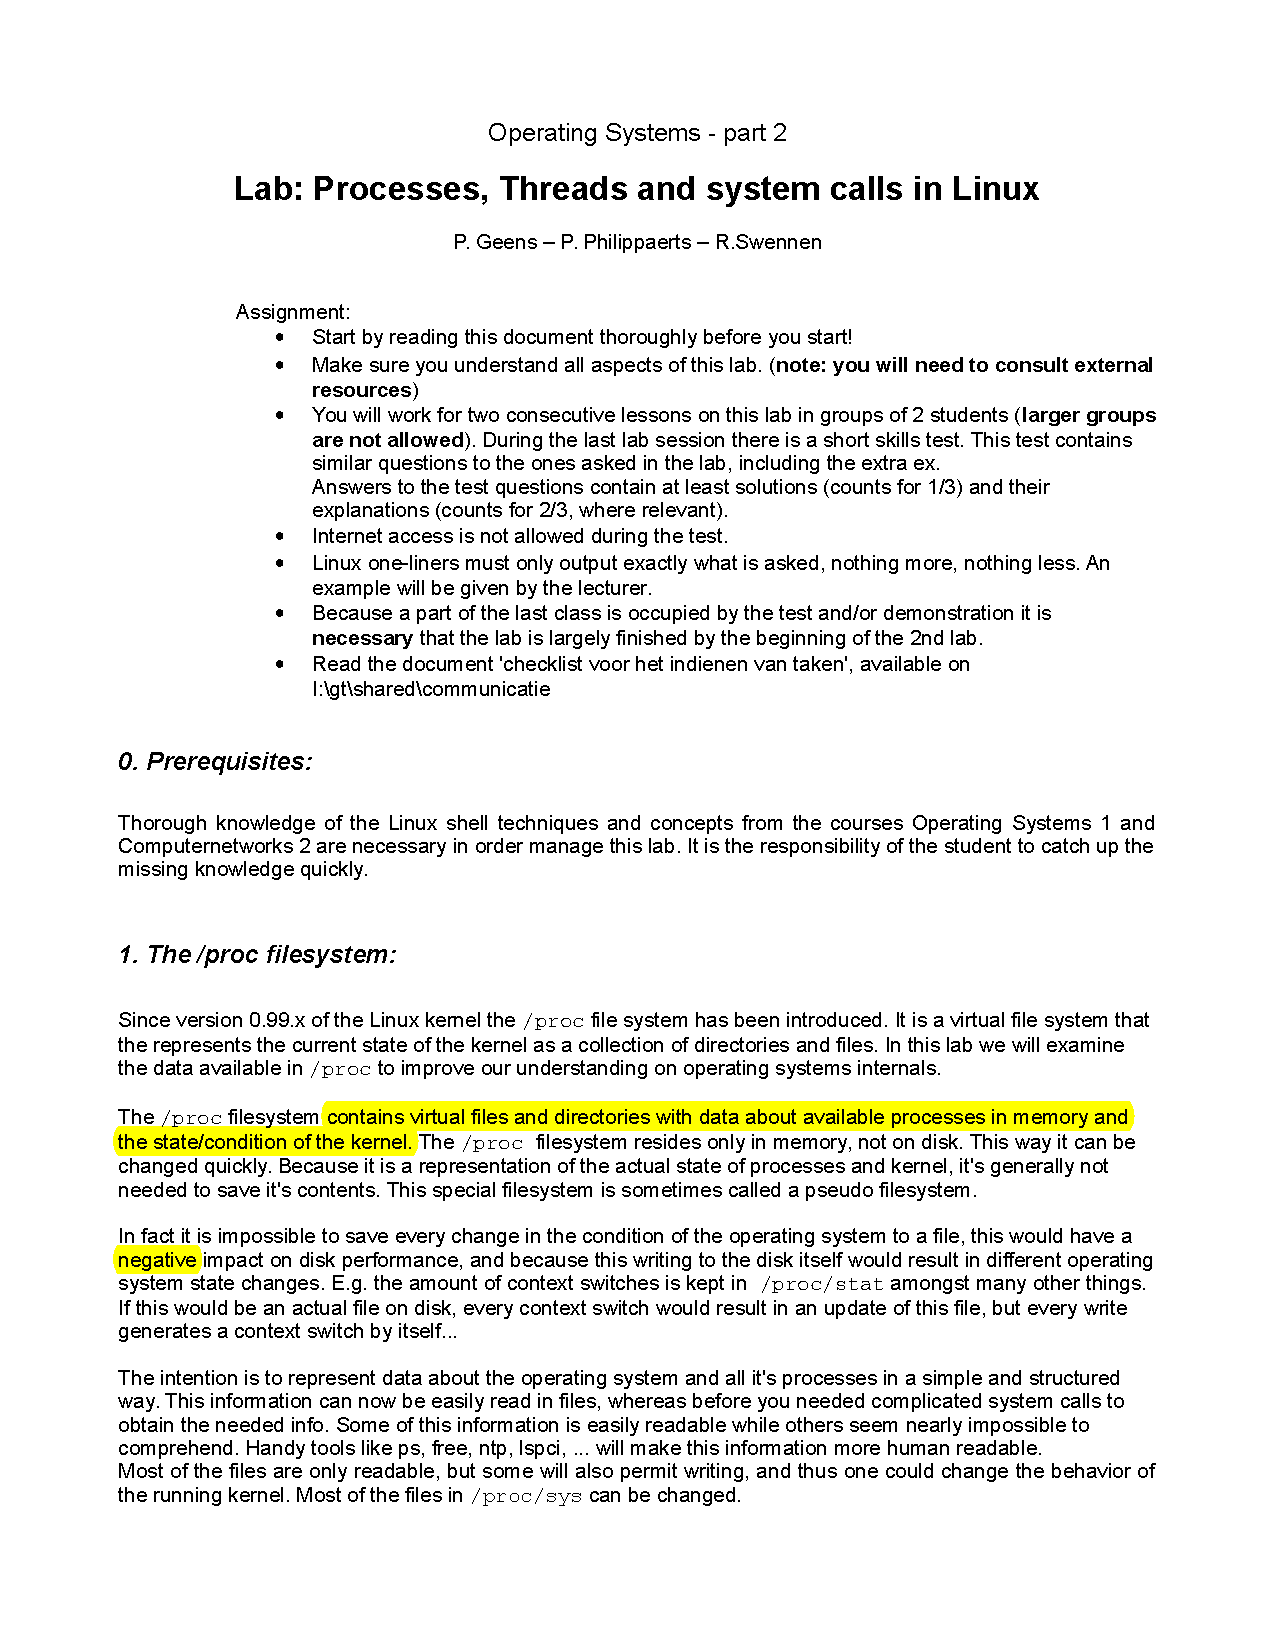
\includepdf[pages=-]{pdf/lab_1_linux_processes_threads_systemcalls}

%hoofdstuk 4
%\setcounter{section}{6}
%\newpage
%\section{Multimedia netwerken}

%\import{sections/lessen/}{1informatiesystemen.tex}

%\stopcontents[chapters]
%\printcontents[chapters]{l}{0}



\part{Examenwiki}
%\startcontents[parts]

\PartialTocPart


\chapter{examenwiki vragen}
%\startcontents[chapters]
%\PartialToc
%\import{sections/examenwiki/}{barrezeele.tex}



%Next we are adding the additional lists to the end of the document:


\clearpage
\part{Glossary}
\PartialTocPart

%\printglossaries
\printglossary[title=Termen,toctitle=Lijst van termen]

\printglossary[type=\acronymtype]


\clearpage
%\import{./}{bibliography.tex}
%\printsolutions

\end{document} 